% !TeX root = main.tex

\noindent\textbf{--\ Response to Reviewer $\sharp1$}\\

\textsf{To minimize the environmental impact of data centers, it is imperative to make data centers more energy efficient while maintaining a high quality of service (QoS). For evaluating the QoS of a data center, an analytical model using queueing theory is proposed. Based on this model, a domain-specific evolutionary optimization framework is developed for finding the optimal placement of virtual network functions in a data center that optimizes multiple conflicting objectives with regard to energy consumption and QoS.}

\textsf{There are some comments about this paper as follows.}

\begin{enumerate}
      \item \textsf{Is the relationship of the five constraints mutually independent or coupling?}\\
            \textcolor{blue}{\textbf{\textit{Reply}: We thank the reviewer for this suggestion. In the updated manuscript we elaborate further on the effect that these constraints have on the difficulty of the problem.}}\\
            \textcolor{blue}{\textit{``The combination of the constraints and objectives results in a challenging optimization problem. Although each of the constraints can be considered independently, each constraint is complex such that the feasible search space is small relative to the overall search space. Further, the NP-Hardness of the problem means that the feasible search space still contains many solutions, few of which will be at or near optimal."} \textbf{(Page x, highlighted in \textcolor{red}{red} color.)}}\\

      \item\textsf{Why do the authors design two tailored features in terms of a solution representation and an initialization operator? Not other tailored features? Please give reasons.}\\
            \textcolor{blue}{\textbf{\textit{Reply}: We thank the reviewer for this suggestion. In the process of our research we explored several alternative mutation and crossover operators but did not find any operators that led to significant improvements. Given the length of the manuscript currently, we did not consider these null results significant enough to include. In light of this comment, we have included some further explanation in the updated manuscript.}}\\
            \textcolor{blue}{\textit{``Further, we found the classic uniform crossover and mutation reproduction operators to be sufficient to vary and exchange information on the number and position of service instances."} \textbf{(Page x, highlighted in \textcolor{red}{red} color.)}}\\

      \item\textsf{Did you try other kinds of solution representations? Is it a genotype-phenotype solution representation suitable for the problem? Why?}\\
            \setItemnumber{5}
            \vspace{-2em}
      \item\textsf{Could you give the specific reasons why the binary and direct solution representations are only able to obtain feasible solutions to small data centers? And why can the proposed solution representation work? What is the essential difference?}\\
            \textcolor{blue}{\textbf{\textit{Reply}: We address comments 3 and 5 together. In the updated manuscript we have moved the comparison of different solution representations to a dedicated subsection with additional analysis.}}\\
            \textcolor{blue}{\textit{
                        ``To answer RQ3, we compare the quality of solutions obtained when different solution representations are applied to the VNFPP. Specifically, the following two meta-heuristic algorithms use NSGA-II as the baseline but have different solution representations.
                        \begin{itemize}
                              \item\underline{Binary representation}: As in [TODO], [TODO], [TODO], a string of binary digits are used to represent if a VNF is assigned to a server.
                              \item\underline{Direct representation}: As in [TODO], a solution is directly represented as a string of VNFs.
                        \end{itemize}
                        In our experiments, we generate $30$ VNFPP instances for six data centers with different sizes. To compare the performance of different algorithms, we use the QoS model developed in Section IV to evaluate the objective functions of the solutions obtained by different algorithms and use the HV indicator as the performance measure."
                  }}
            \begin{figure}[t!]
                  \centering
                  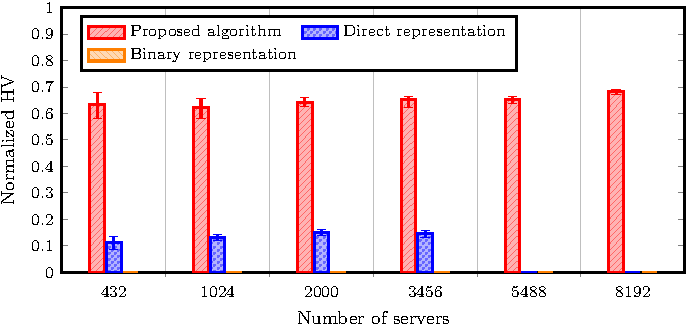
\includegraphics[width=.75\linewidth]{figs/comparison-crop}
                  \caption{The lower quartile, median, and upper quartile of the hyper-volume of the population for different algorithms on 30 VNFPP instances found by NSGA-II using different solution representations on 30 VNFPP instances}
            \end{figure}
            \begin{figure}[t!]
                  \centering
                  \begin{subfigure}[b]{0.3625\linewidth}
                        \includegraphics[width=\textwidth]{figs/qm-crop}
                        \caption{Proposed algorithm}
                  \end{subfigure}
                  \begin{subfigure}[b]{0.3625\linewidth}
                        \includegraphics[width=\textwidth]{figs/std-crop}
                        \caption{Direct representation}
                  \end{subfigure}

                  \vspace{1em}
                  \caption{An illustrative example of the final populations found by NSGA-II using our proposed representation and the direct solution representation. The binary solution representation is omitted as it resulted in no feasible solution at all.}
                  \label{fig:solution_representation_objectives}
            \end{figure}

            \textcolor{blue}{\textit{
                        ``From the results shown in Figs.~\ref{fig:solution_representation_comparison} and~\ref{fig:solution_representation_objectives}, we find that the solutions obtained by our proposed solution representation significantly outperform alternative representations. Our proposed solution representation has two advantages over existing representations. First, our proposed representation guarantees feasible solutions irregardless of the input. In contrast, both the direct and binary solution representations were unable to find feasible solutions to larger problem instances. Second, our proposed representation integrates domain knowledge to generate solutions with shorter average distances between VNFs causing the resultant solutions to be closer to the Pareto front than alternative representations. Existing solution representations do not utilize this information and instead rely solely on the optimization framework to locate high quality solutions.\\
                        Although the binary solution representation has been successfully applied to solve the VNFPP on small data centers (e.g.,~\cite{ChantreF20,KaurGK020,CharismiadisTPM20}), it does not scale well in the larger-scale problems considered in our experiments. With a binary solution representation, multiple VNFs to be placed on the same VM. This greatly complicates the search process compared to the direct or proposed solution representations with which this constraint is impossible to violate.\\
                        The direct solution representation is also only able to obtain feasible solutions to small data centers, as shown in~\pref{fig:alg_objectives}, and exclusively finds solutions with high energy consumption. In particular, since a solution is only feasible when there is an instance of each VNF, solutions with more VNFs are more likely to be feasible than those with less VNFs and lower energy consumption. This leads the algorithm with the direct representation to be biased towards solutions with a high energy consumption. On larger problems with high numbers of VNFs, the direct solution representation is unable to find a solution with at least one instance of each VNF."
                  } \textbf{(Page x, highlighted in \textcolor{red}{red} color.)}}\\
            \setItemnumber{4}

      \item\textsf{Section VI.B, p.9, “we apply our initialization operator to generate 100 randomly generated candidate solutions for each problem.”?}\\
            \textcolor{blue}{\textbf{\textit{Reply}: We apologize for the lack of clarity in this sentence. In the updated manuscript, this sentence reads as follows.}}\\
            \textcolor{blue}{\textit{``To create the benchmark, we generate 100 VNFPP problems for a data center with 412 servers to constitute a diverse set of
                        problems. Then, we use our proposed initialization operator (see Section V-B) to generate 100 candidate solutions for each problem."} \textbf{(Page x, highlighted in \textcolor{red}{red} color.)}}\\

            \setItemnumber{6}
      \item\textsf{Which key components of the proposed tailored EMO algorithm play roles to obtain solutions in terms of both convergence and diversity? Please give more discussions and analyses.}\\
            \textcolor{blue}{\textbf{\textit{Reply}: We thank the reviewer for this suggestion. In the updated manuscript, we elaborate further on the contributions of each of our tailored operators.}}
            \begin{figure*}[t!]
                  \centering
                  \begin{subfigure}[b]{0.32\linewidth}
                        \includegraphics[width=\textwidth]{figs/comparison/qm-crop}
                        \caption{Proposed algorithm}
                  \end{subfigure}
                  \begin{subfigure}[b]{0.32\linewidth}
                        \includegraphics[width=\textwidth]{figs/comparison/std-crop}
                        \caption{Direct representation}
                  \end{subfigure}

                  \vspace{1em}

                  \begin{subfigure}[b]{0.32\linewidth}
                        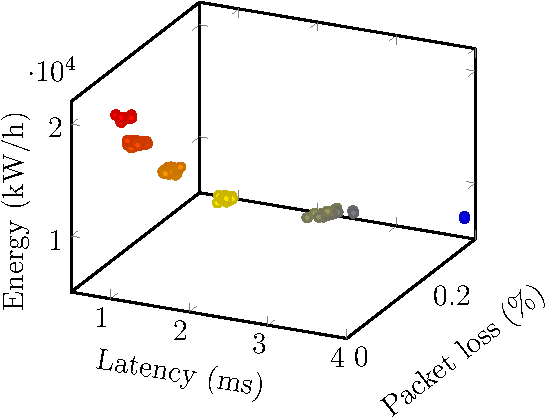
\includegraphics[width=\textwidth]{figs/comparison/esp_vdce-crop}
                        \caption{ESP-VDCE \cite{TODO}}
                  \end{subfigure}
                  \begin{subfigure}[b]{0.32\linewidth}
                        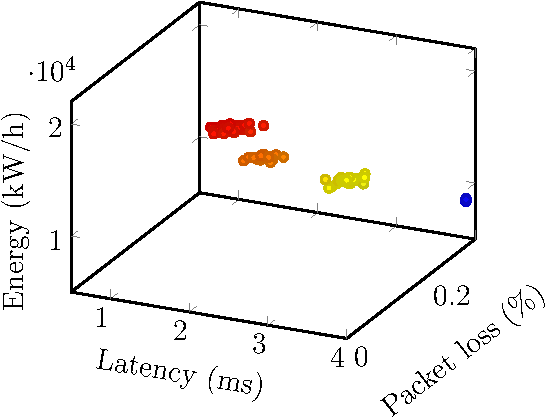
\includegraphics[width=\textwidth]{figs/comparison/bfdsu-crop}
                        \caption{BFDSU \cite{TODO}}
                  \end{subfigure}
                  \begin{subfigure}[b]{0.32\linewidth}
                        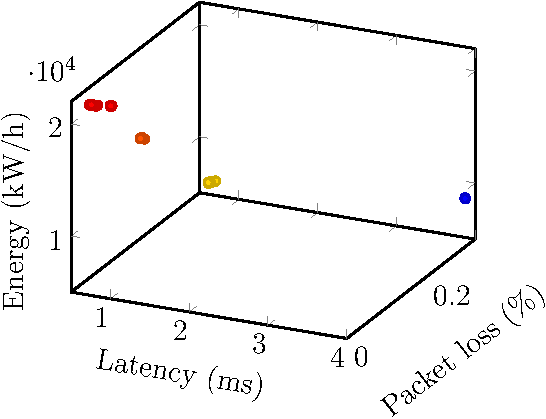
\includegraphics[width=\textwidth]{figs/comparison/stringer-crop}
                        \caption{Stringer \cite{TODO}}
                  \end{subfigure}

                  \vspace{1em}
                  \caption{An illustrative example of the objective values of the solutions in the final populations found by NSGA-II using our proposed algorithm and algorithms from the literature. Subproblems for the heuristic were generated using our proposed initialization operator. The binary solution representation is omitted as it resulted in no feasible solution at all.}
                  \label{fig:alg_objectives}
            \end{figure*}
            \begin{figure*}
                  \centering
                  \hfill
                  \begin{minipage}[t]{.48\textwidth}
                        \centering
                        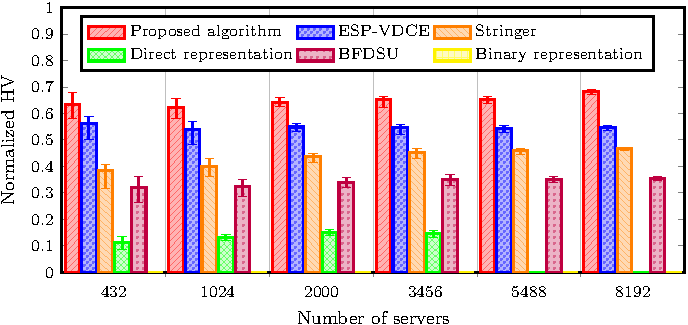
\includegraphics[width=\columnwidth]{figs/comparison/comparison-crop}
                        \caption{The lower quartile, median, and upper quartile of the hyper-volume of the population for different algorithms on 30 VNFPP instances using the initialization operator to generate subproblems for the heuristics.}
                        \label{fig:alg_comparison}
                  \end{minipage}\hfill
                  \begin{minipage}[t]{.48\textwidth}
                        \centering
                        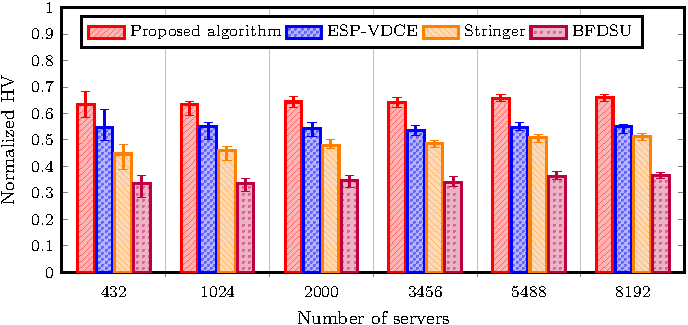
\includegraphics[width=\columnwidth]{figs/comparison/alg_fixed-crop}
                        \caption{The lower quartile, median, and upper quartile of the hyper-volume of the population for different algorithms on 30 VNFPP instances using the solutions of our proposed algorithm to generate subproblems for the heuristics.}
                        \label{fig:alg_fixed}
                  \end{minipage}
                  \hfill
            \end{figure*}\\
            \textcolor{blue}{\textit{
                        ``From the results shown in~\pref{fig:alg_comparison} and~\pref{fig:alg_fixed}, it is clear that our proposed algorithm outperforms other competitors on all test cases. This can be attributed to our two proposed operators. First, it is clear from \pref{fig:alg_objectives} that proposed operators enable a diverse population of solutions. Our two proposed operators work together towards this goal. The initialization operator produces a diverse range of possible solutions, whilst the solution representation ensures that these solutions are feasible.\\
                        Second, our proposed solution representation minimizes the distance between sequential VNFs, improving the overall QoS. We note that the two best performing algorithms, our proposed algorithm and ESP-VDCE, aim to minimize the distance between sequential VNFs. In contrast, both BFDSU and Stringer tend to produce longer path lengths thus lead to significantly worse solutions than our proposed algorithm. Since Stringer restricts the capacity of each server, it causes services to be placed across multiple servers. Likewise, the stochastic component of BFDSU can cause it to place VNFs far away from any other VNF of the service. In contrast, our proposed algorithm incorporates useful information into the optimization process and places sequential VNFs close by thus leading to better solutions.\\
                        A final benefit of our algorithm is that it can iteratively improve the placements to minimize the energy consumption and QoS. Although ESP-VDCE does consider the path length, it otherwise uses a simple first fit heuristic that cannot consider how service instances should be placed in relation to each other. As a consequence, the performance of ESP-VDCE depends on the order in which services are considered. Our proposed algorithm considers the problem holistically and can make informed placement decisions."}\textbf{(Page x, highlighted in \textcolor{red}{red} color.)}}\\

      \item\textsf{What are disadvantages of the proposed algorithm? Give them in Section VII.}\\
            \textcolor{blue}{\textbf{\textit{Reply}: We thank the reviewer for this suggestion. In the updated manuscript, we conclude with a discussion of the weaknesses and potential improvements of our proposed algorithm.}}\\
            \textcolor{blue}{\textit{``There are some disadvantages and extensions to our current approach that could be considered in future work.
                        \begin{itemize}
                              \item A limitation of our proposed algorithm is that it is only applicable to Fat Tree network topologies. However, the underlying heuristic of our work - prefer to place VNFs on nearby servers - is applicable to any data center. It would be interesting to extend this work to arbitrary topologies.
                              \item Although execution time is not a priority in this work, it is notable that metaheuristic approaches are typically slower than heuristic algorithms since they requires a large number of model evaluations. That said, the significant improvements we make over existing heuristic alternatives justifies our approach. In future work, fast heuristic alternatives to accurate models may reduce this gap between heuristic and metaheuristic algorithms.
                              \item Furthermore, there are interesting possibilities in exploring the impact of different types of VNF and service. It would be interesting to determine how an alternative problem formulation would affect the design and results of a meta-heuristic alternative."
                        \end{itemize}} \textbf{(Page x, highlighted in \textcolor{red}{red} color.)}}
\end{enumerate}

\clearpage
